\documentclass[12pt]{standalone}

\usepackage{tikz,etoolbox}
\usetikzlibrary{arrows.meta, positioning, shapes, shapes.geometric, calc}

\usepackage{tikz}
\usetikzlibrary{arrows.meta, positioning, shapes}

% Sanserif font:
\renewcommand{\familydefault}{\sfdefault}

% Attempt to get a little border padding
% \usepackage[
%     left=0.20in,
%     right=0.20in,
%     top=0.20in,
%     bottom=0.20in,
% ]{geometry}



\begin{document}

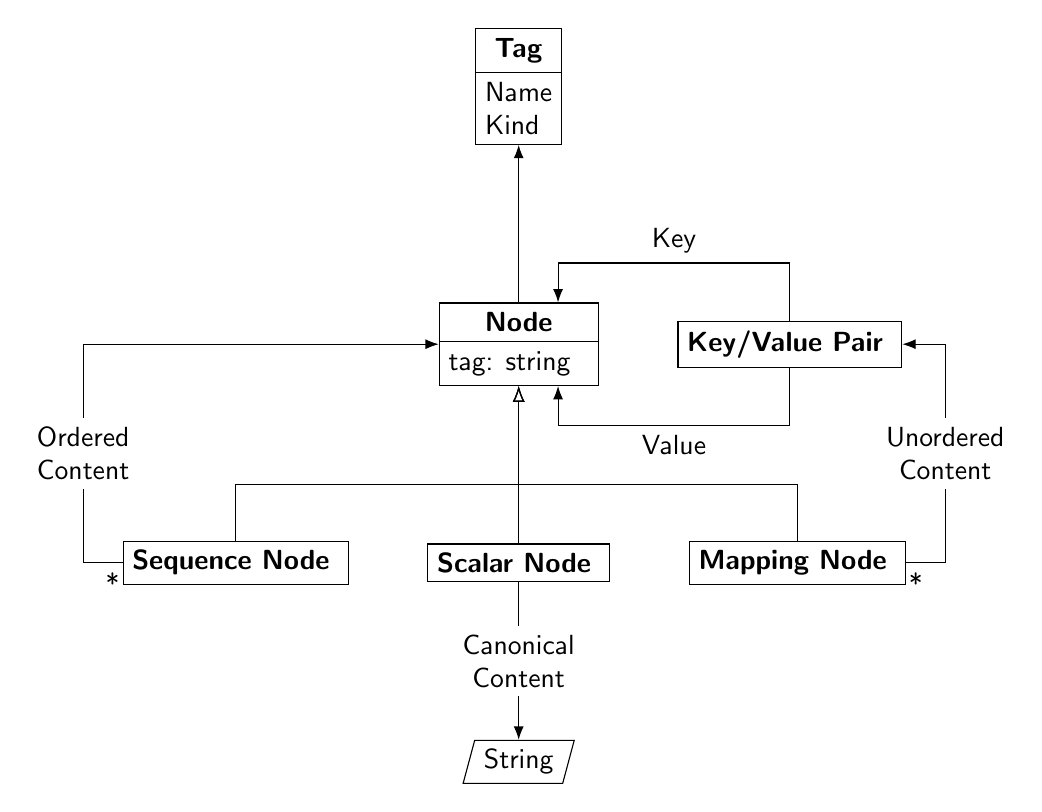
\begin{tikzpicture}[
    entity/.style = {
        draw,
        rectangle,
        anchor=north,
    },
    entityAttrs/.style = {
        entity,
        rectangle split,
        rectangle split parts=2,
    },
    parallellogram/.style = {
        draw,
        trapezium,
        trapezium left angle=75,
        trapezium right angle=105,
    },
    onArrow/.style = {
        fill=white,
        align=center,
    },
    has/.style = {
        -{Latex},
    },
    inherits/.style = {
        -{Latex[open, length=2mm]},
    },
    node distance=2cm and 1cm,
]

\newcommand{\entity}[3][]{
    \node(#2)[
        \ifstrempty{#3}{entity}{entityAttrs},
        #1
    ] {
        \textbf {#2}
        \ifstrempty{#3}{}{
            \nodepart[align=left]{second} #3
        }
    };
}

\entity{Node}{tag: string};

\entity[above=of Node]{Tag}{Name\\Kind};
\draw[has] (Node) -- (Tag);

\entity[below=of Node]{Scalar Node}{};
\draw[inherits] (Scalar Node) -- (Node);

\node[parallellogram, below=of Scalar Node](Canonical Content) {String};
\draw[has] (Scalar Node) -- (Canonical Content)
    node[onArrow, midway] {Canonical\\Content};

\entity[left=of Scalar Node]{Sequence Node}{};
\draw[inherits] (Sequence Node) -- ++(0,+10mm) -| (Node);

\draw[has] (Sequence Node.west) -- ++(-5mm, 0) node[near start, below] {*}
    |- (Node) node[onArrow, pos=0.25] {Ordered\\Content};

\entity[right=of Scalar Node]{Mapping Node}{};
\draw[inherits] (Mapping Node) -- ++(0,+10mm) -| (Node);

\entity[right=of Node]{Key/Value Pair}{};

\draw[has]
    (Mapping Node.east) -- node[near start, below] {*}
    ++(5mm, 0) |- (Key/Value Pair) node[onArrow, pos=0.25] {Unordered\\Content};

\draw[has] (Key/Value Pair.north)
    |- ($(Node.north)+(0.5,0.5)$)
    node[pos=0.75, above] {Key}
    -- ($(Node.north)+(0.5,0)$);

\draw[has] (Key/Value Pair.south)
    |- ($(Node.south)+(0.5,-0.5)$)
    node[pos=0.75, below] {Value}
    -- ($(Node.south)+(0.5,0)$);

\end{tikzpicture}

\end{document}
